\documentclass[a4paper, 11pt]{article}
\usepackage[a4paper, left=1in, right=1in, top=1in, bottom=1in]{geometry}
\usepackage[dvipsnames]{xcolor}
\usepackage{graphicx} % Required for inserting images
\usepackage{amsfonts}
\usepackage{amssymb}
\usepackage{amsmath}
\usepackage{tikz,lipsum,lmodern}
\usepackage[most]{tcolorbox}
\usepackage{pgfplots}
\usepackage{tabularx}
\usepackage{stmaryrd}
\usepackage{tikz} 
\usepackage{imakeidx}
\usepackage{blindtext}
\usepackage{hyperref}
\usepackage[rightcaption]{sidecap}
\usepackage{wrapfig}
\usepackage{cancel}
\usepackage{titlesec}
\usepackage{enumitem}
\usepackage{float}
\usepackage{tabularx}
\usepackage{adjustbox}
\usepackage{multicol}
\usepackage{listings}
\usepackage{longtable}
\setlist{nolistsep} % Rimuove lo spazio extra tra gli elementi della lista

\definecolor{comment}{rgb}{0.5, 0.5, 0.5}
\definecolor{string}{rgb}{0.3, 0.6, 0.3}
\definecolor{keyword}{rgb}{0.7, 0, 0.4}
\definecolor{identifier}{rgb}{0.2, 0.2, 1}
\definecolor{background}{rgb}{0.99, 0.99, 0.99}

\lstdefinelanguage{SQL}{
    morekeywords={
        SELECT, INSERT, UPDATE, DELETE, FROM, WHERE, AND, OR, NOT, IN, AS, JOIN,
        ON, CREATE, DROP, TABLE, DATABASE, ALTER, ADD, CONSTRAINT, PRIMARY, KEY,
        FOREIGN, IF, NULL, DEFAULT, AUTO_INCREMENT, INDEX, VALUES, INTO, THEN
    },
    sensitive=false,
    morecomment=[l]{--},
    morecomment=[s]{/*}{*/},
    morestring=[b]',
    morestring=[b]"
}


\lstset{
    basicstyle=\ttfamily,
    keywordstyle=\color{keyword},
    commentstyle=\color{green},
    stringstyle=\color{string},
    numbers=left,
    numberstyle=\tiny\color{gray},
    stepnumber=1,
    numbersep=10pt,
    backgroundcolor=\color{white},
    showspaces=false,
    showstringspaces=false,
    breaklines=true,
    frame=single,
    frameround=tttt
}

\lstdefinestyle{customcpp}{
    language=C++,
    basicstyle=\ttfamily\footnotesize,
    backgroundcolor=\color{background},
    keywordstyle=\color{keyword},
    identifierstyle=\color{identifier},
    commentstyle=\color{comment}\itshape,
    stringstyle=\color{string},
    numbers=left,
    numberstyle=\tiny\color{gray},
    stepnumber=1,
    numbersep=10pt,
    tabsize=4,
    showspaces=false,
    showstringspaces=false,
    breaklines=true,
    breakatwhitespace=true,
    escapeinside={\%*}{*)},
    frame=single,
    rulecolor=\color{black},
    captionpos=b,
    morekeywords={override, nullptr},
}
\titleformat{\chapter}[display]
  {\normalfont\Large\bfseries} % Stile del titolo
  {\chaptername\ \thechapter}{10pt}{\Large}

\hypersetup{
    colorlinks=true,
    linkcolor=black,
    filecolor=magenta,      
    urlcolor=blue,
    pdftitle={Relazione_Centro-Controllo-Droni},
    pdfpagemode=FullScreen,
}


\makeindex[columns=3, title=Alphabetical Index, intoc]


\newcommand\scalemath[2]{\scalebox{#1}{\mbox{\ensuremath{\displaystyle #2}}}}


\title{Relazione su \\
Controllo formazione droni}
\author{A. Bettoni (1998044),\\ A. Coppola (2003964),\\S. Di Cesare (1938649)}
\date{\today}

\begin{document}
\maketitle
\newpage
\tableofcontents
\newpage
\section{Descrizione Generale}
\paragraph*{Problema:}
Si vuole progettare un sistema di controllo di n droni che sorvegli una data area rettangolare.
Il sistema deve garantire che, con i droni forniti, ogni punto dell'area venga sorvegliato il più frequentemente possibile.

I droni partiranno dalla torre di controllo che si trova al centro dell'area da sorvegliare.
Ogni drone ha un'autonomia limitata (misurata in minuti in volo) e una velocità massima. 
La torre dovrà gestire gli spostamenti di ogni drone facendo in modo che tornino alla torre prima che la batteria sia del tutto esaurita. 
Quando i droni si trovano nella torre di controllo sono considerati in carica e il tempo di ricarica può variare da drone a drone.

\paragraph*{Dati sperimentali:}
Si assume che:
\begin{enumerate}
    \item Ogni drone si muove alla velocità costante di $30\ km/h$
    \item Il tempo di ricarica varia tra le 2 e le 3 ore 
    \item Un punto si dice visitato se si trova nel raggio di 10 m da un drone
\end{enumerate}
\paragraph*{Idea di soluzione:}
Abbiamo scelto di modellare il problema con un sistema che agisce sulla torre di controllo e ricarica che a sua volta controlla i droni.
Dunque la torre invia ad ogni drone le coordinate del punto sull'area da raggiunge secondo un sistema di volo a "tappe".
Una volta che il drone arriva alla posizione ricevuta lo comunica alla torre che risponde con la posizione successiva, delineando così un percorso.
Quando il drone è scarico lo comunica alla torre e si direziona alla torre di controllo, per essere ricaricato.

Sta al sistema quindi il compito di calcolare, mentre i droni sono in volo, il percorso migliore per far sì che ogni punto dell'area venga sorvegliato 
il più frequentemente possibile, tenendo conto dei punti visitati, dei droni in volo, e dei punti che visitano prima di scaricarsi.
\begin{figure}[h]
    \centering
    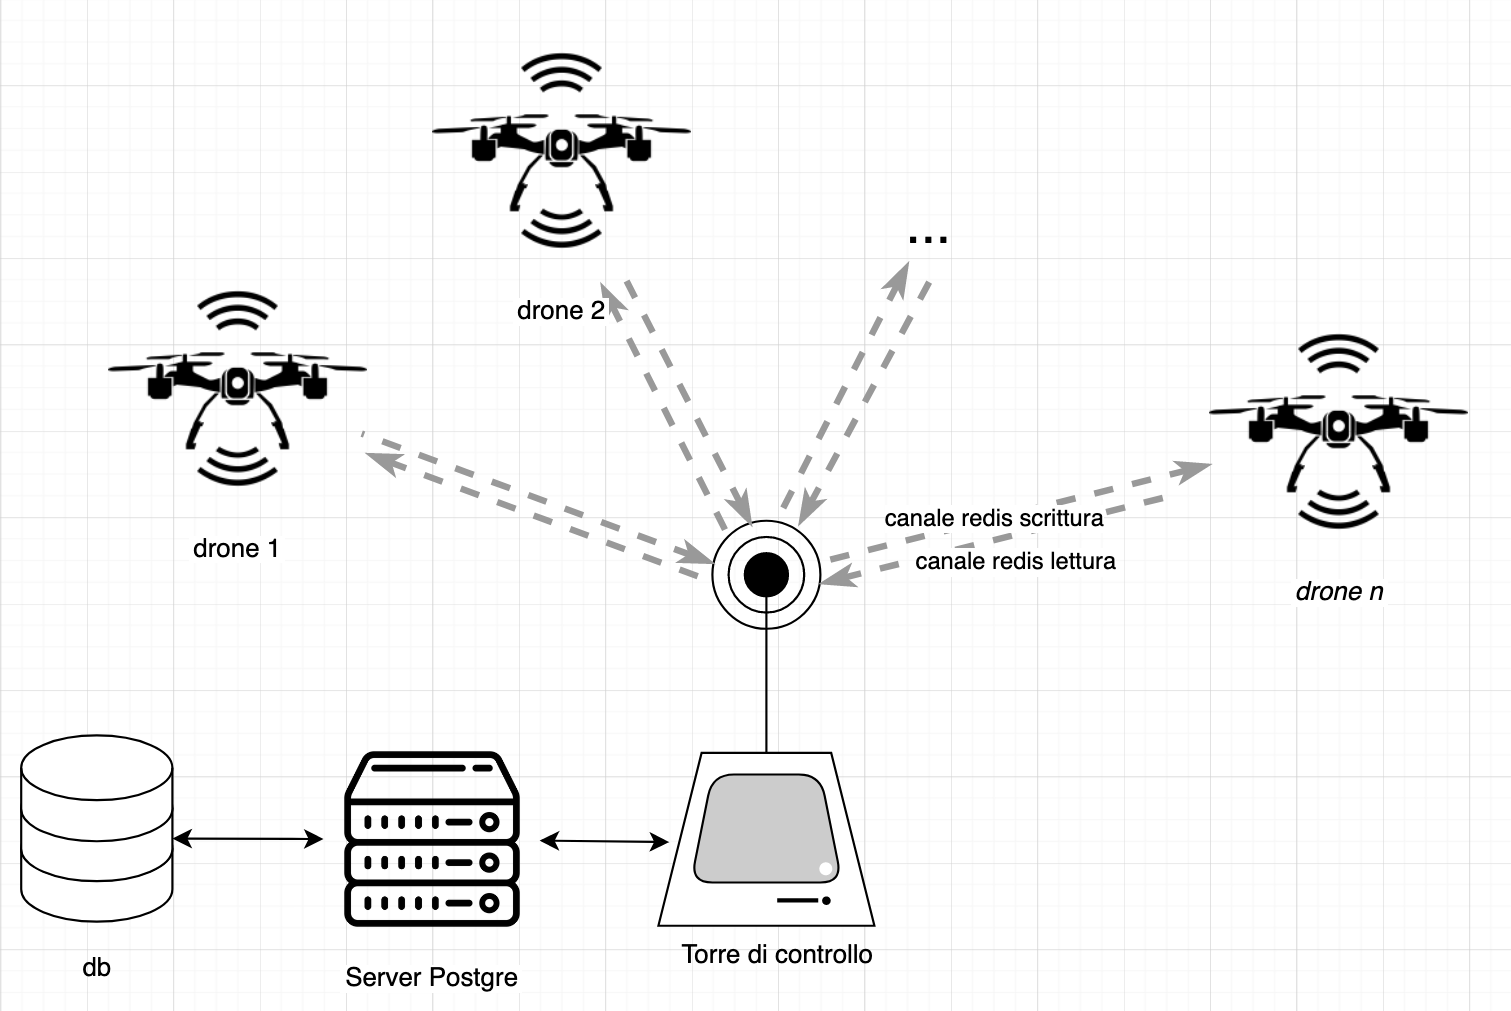
\includegraphics[height = 7.2 cm]{image/Architettura.png}\\
    \caption{Architettura fisica del sistema}
\end{figure}
\newpage

\section{Analisi del software}
\subsection{Requisiti utente}
Per funzionare, il sistema ha bisogno dei seguenti requisiti:
\begin{itemize}
    \item dimensione dell'area\\
    Ogni punto dell'area è identificato dalla sua posizione in una matrice di punti e di quei punti ci interessa solo:
    \begin{itemize}
        \item il tempo trascorso dall'ultima visita.
    \end{itemize}
    \item numero di droni\\
    per ogni drone è di interesse:
    \begin{itemize}
        \item Stato : tra i stati precedentemente elencati
        \item posizione 
        \item carica residua (in minuti)
        \item carica massima (in minuti)
        \item tempo di ricarica 
        \item last\_update : tempo trascorso dall'ultimo update
    \end{itemize}
    
\end{itemize}
\subsection{Requisiti di sistema}
Il sistema deve rispettare i seguenti requisiti:
\begin{enumerate}
    \item Area:
    \begin{enumerate}[label=1.\arabic*]
        \item I blocchi sono tutti tra loro disgiunti (non esiste un punto dell'area che si trova in più di un blocco)
        \item L'unione dei blocchi copre tutti e solo i punti dell'area (un punto appartiene all'area se e solo se esiste un blocco che lo contiene)
        \item Un blocco può essere assegnato al più ad un drone 
    \end{enumerate}
    \item Drone:
    \begin{enumerate}[label=1.\arabic*]
        \item Un drone a cui è stato assegnato un blocco può trovarsi al di fuori di esso se e solo se:
        \begin{enumerate}
            \item il drone è partito dalla torre e si sta posizionando verso il punto di partenza del blocco
            \item il drone è scarico e sta tornando alla torre
            \item il drone ha visitato tutto il blocco e si sta posizionando verso il punto di partenza di un'altro blocco
        \end{enumerate}
        \item Un drone può volare verso un punto diverso da quello della torre se e solo se il suo tempo di volo residuo è maggiore del tempo che serve al drone per tornare alla torre \textit{(più un valutato margine di errore)}
    \end{enumerate}
    \item Torre:
    \begin{enumerate}[label=1.\arabic*]
        \item La torre non può terminare il suo processo se esiste un drone connesso che non è tornato nella torre di controllo.
        \item Tutti i punti che la torre invia ad un drone devono trovarsi all'interno dell'area assegnata al drone
    \end{enumerate}
    \item Requisiti non-funzionali:
    \begin{enumerate}[label=1.\arabic*]
        \item ogni punto dell'area deve essere visitato il più frequentemente possibile
        \item Il tempo di risposta della torre per ogni drone deve essere ragionevolmente basso per fare in modo che i droni rimangano fermi sul posto il meno possibile
    \end{enumerate} 
\end{enumerate}
\newpage

\subsection{Algoritmo}
Contando di poter ottenere per ogni drone, una tupla contenente almeno \{\textit{Id, Posizione, Stato, Blocco}\} di tutti i droni che si sono connessi alla torre e le dimensioni dell'area da sorvegliare, la torre inizia a seguire il seguente algoritmo.
Il problema può essere gestito seguendo i seguenti passaggi:
\begin{enumerate}
    
    \item La torre di controllo conta i droni che si sono connessi e divide l'area da sorvegliare in $N$ blocchi \underline{tutti della stessa misura}
     secondo una specifica funzione approssima per eccesso i blocchi necessari per far volare tutti i droni.

    \item La torre assegna ad ogni drone \textit{"pronto a partire"} un blocco disponibile.

    \item Ogni drone si dirige al punto di partenza del blocco assegnatogli. Non appena lo raggiunge lo comunica alla torre.

    \item Quindi la torre azzera il tempo di visita dell'area $10\sqrt 2\times 10\sqrt 2$ (\textit{la scelta della dimensione verrà approfondita in seguito}) centrata nella posizione del drone e gli invia il prossimo punto da raggiungere
     per scansionare tutto il blocco.

    \item Quando il drone ha visitato tutto il blocco gli viene assegnato il blocco disponibile che contiene il punto non visitato da più tempo. Il loop continua dal punto 3.
    \item Quando un drone ha carica appena sufficiente per tornare alla torre di controllo parte la procedura di return. 
    Segnala alla torre che sta tornando comunica quindi l'ultimo punto visitato e si dirige alla torre.
    
    \item Quando il drone arriva alla torre di controllo inizia a ricaricarsi.
    La torre lo marchera come \textit{"pronto a partire"} non appena la batteria sarà carica.

    \item Se la torre non riceve messaggi da un drone in volo per troppo tempo questo verrà segnato come \textit{"morto"}. 
\end{enumerate}
Questo è l'idea principale per far si che tutti i punti vengano visitati il più frequentemente possibile.
Questo ciclo viene ripetuto finche l'utente non interrompe il programma o tutti i droni "muoiono".
\subsection{Diagrams}
\begin{figure}[htbp]
    \centering
    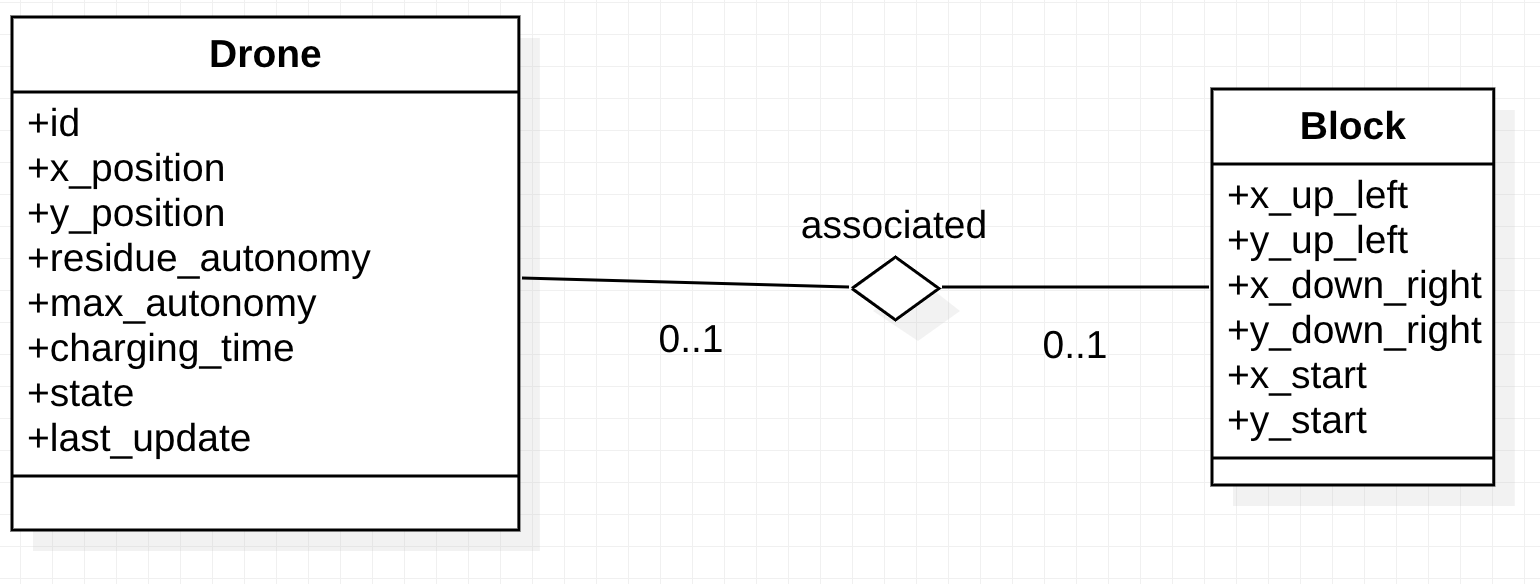
\includegraphics[height = 4 cm]{image/ER.png}%
    \qquad\qquad
    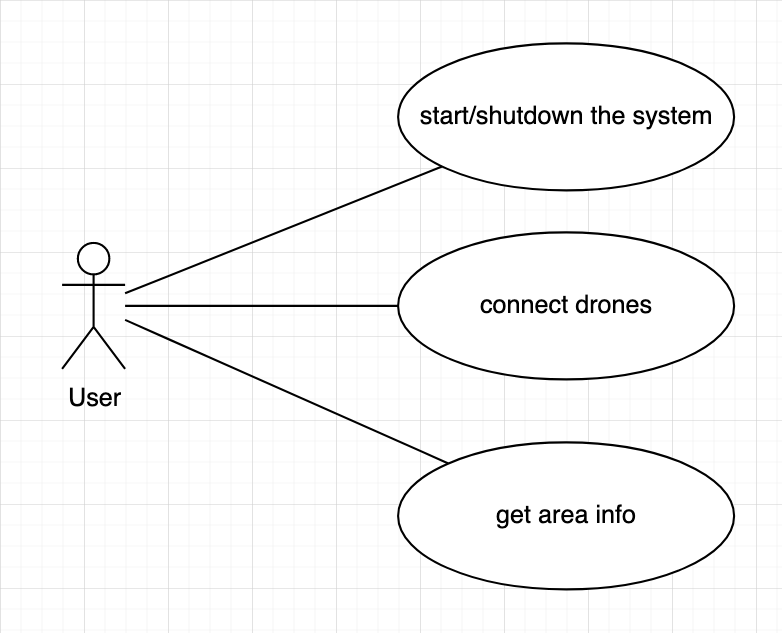
\includegraphics[height = 4 cm]{image/UML1.png}
    \caption{schema ER e UML}
\end{figure}


\begin{figure}[h]
    \centering
    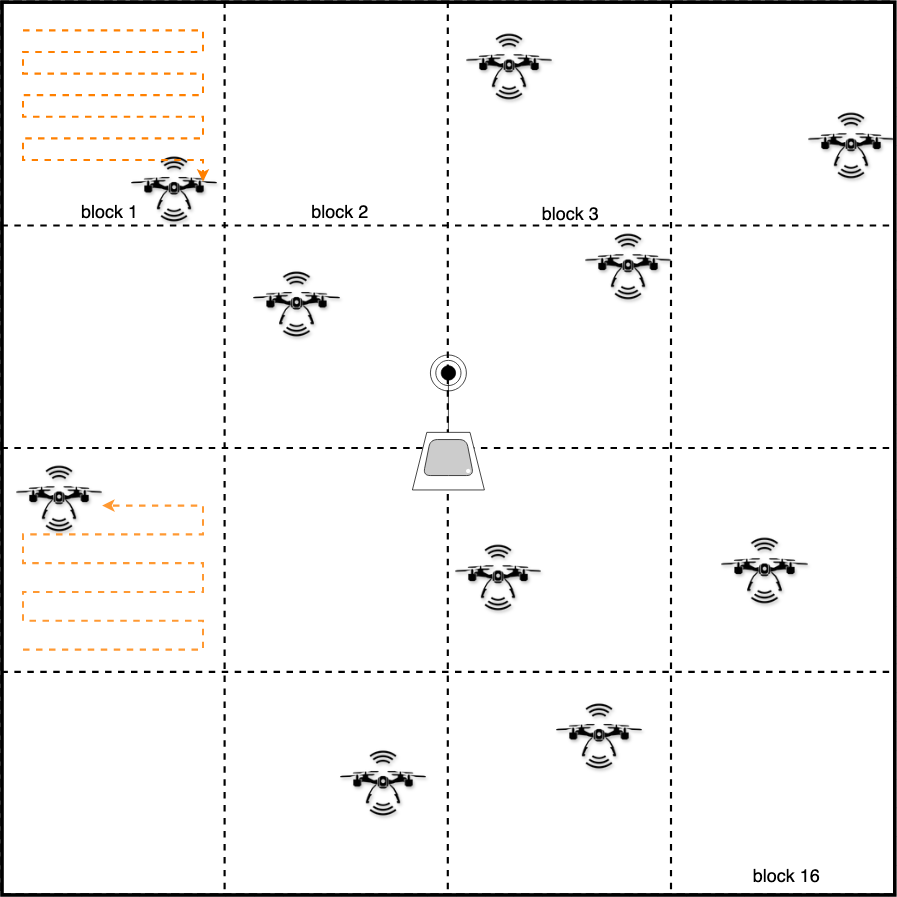
\includegraphics[height = 8 cm]{image/DroniInArea.png}%
    \ 
    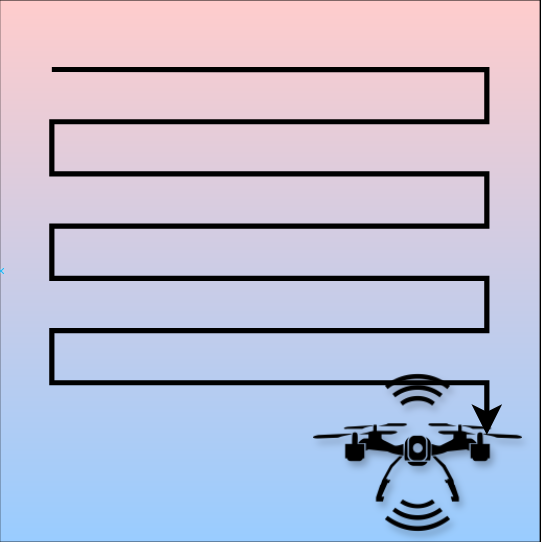
\includegraphics[height = 4 cm]{image/DroneInBlock.png}
    \caption{\small{Esempio di area suddivisa in blocchi. Nel dettaglio a destra oltre al percorso seguito dal drone, viene evidenziata come più "calda" l'area visitata da meno tempo e più "fredda" l'area appena vista.}}
\end{figure}

\begin{figure}[H]
    \centering
    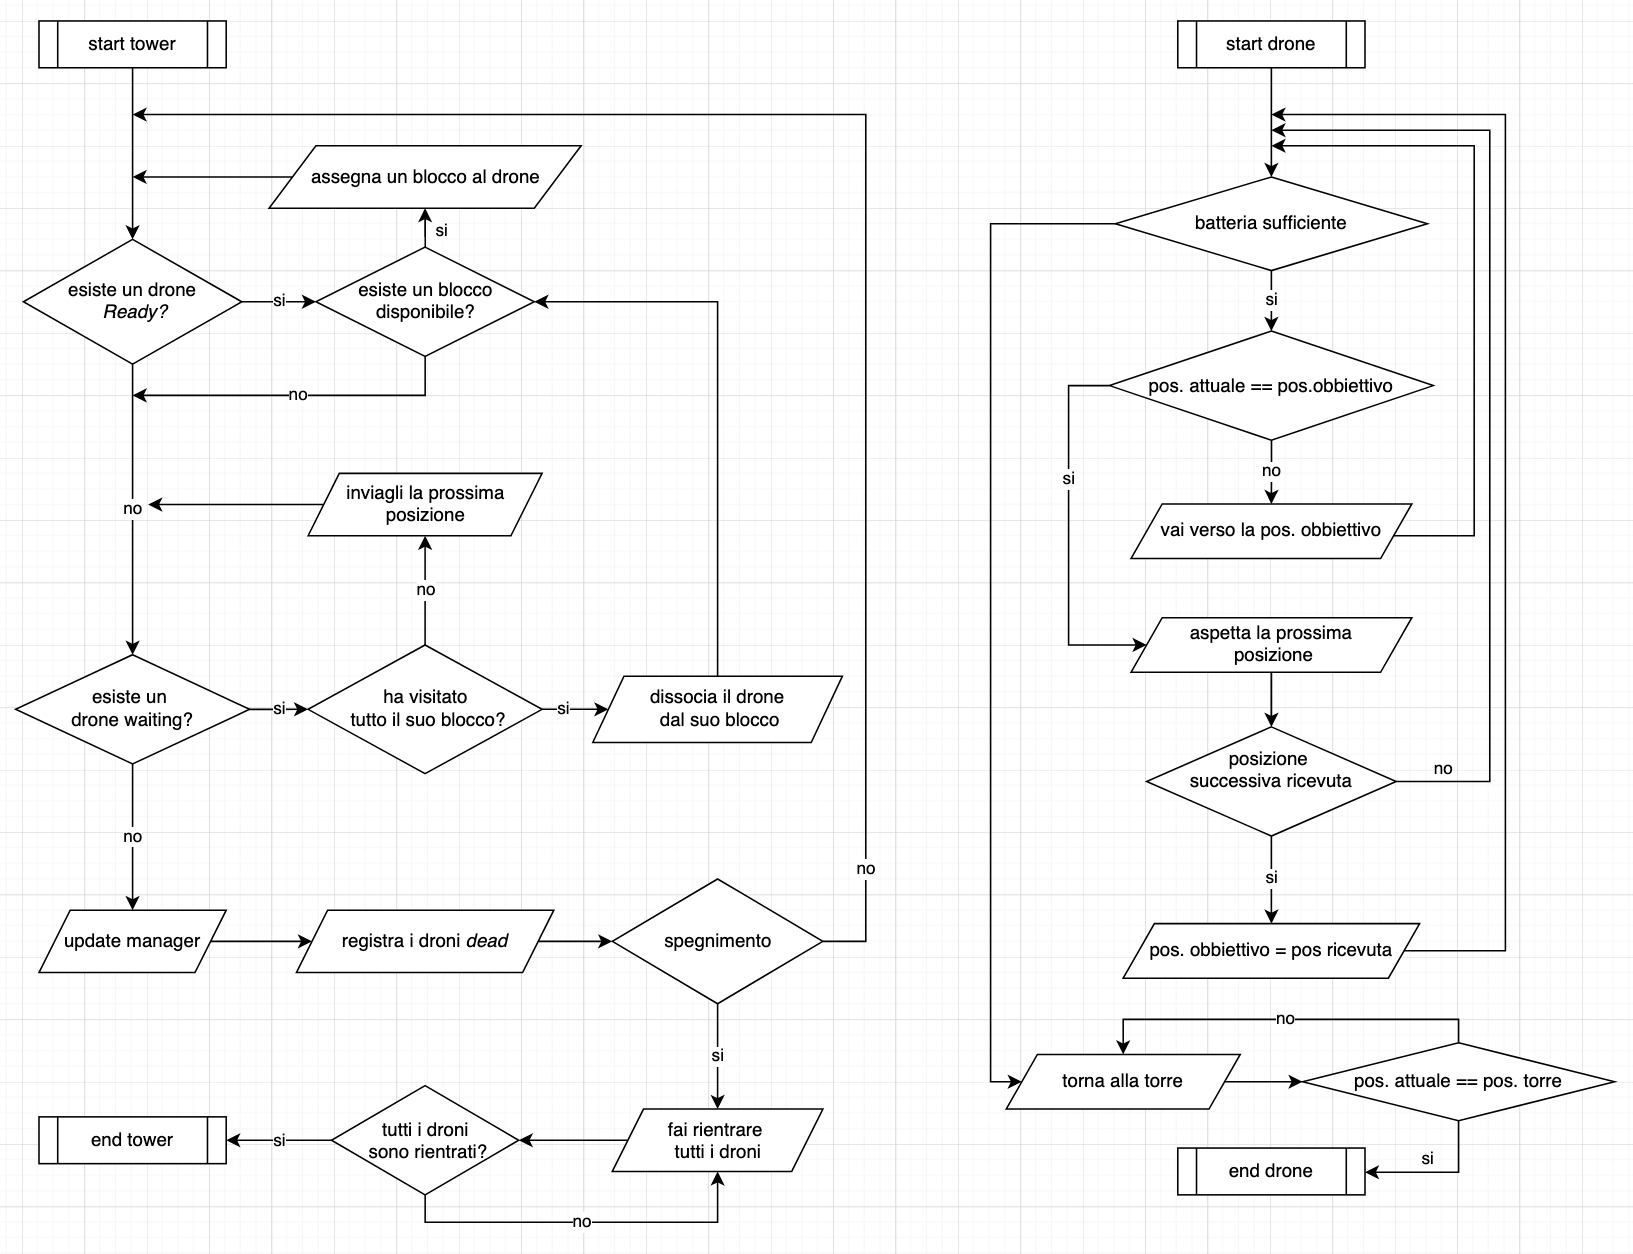
\includegraphics[height = 13 cm]{image/FlowCharts.png}%
    
    \caption{\small{FlowChart della torre e del drone. Nota bene, nel FlowChart viene assunto che il drone e la torre siano già connessi. Il Flow Chart del drone ne rappresenta il ciclo di vita dal momento che parte dalla torre al momento che vi rientra.}}
    
\end{figure}

\begin{figure}[H]
    \centering
    \includegraphics[height = 17 cm]{image/activityDiagram.png}
    \caption{Activity diagram del sistema di interazione e decisione tra torre e drone, nel diagramma sono mostrate due barriere in cui drone e torre si sincronizzano per scambiarsi i messaggi principali mentre è lasciato implicito l'handler message di entrambi per messaggi di check.}
    
\end{figure}


\newpage
\subsubsection{State diagram}
Per decidere l'azione da assegnare ad ogni drone la torre deve riuscire a distinguere la condizione di ogni drone. 
Definiamo quindi $6$ stati in cui ogni drone può trovarsi:
\begin{enumerate}
    \item \textbf{CHARGING:} il drone si trova alla base, e sta ricaricando la sua batteria
    \item \textbf{READY:} il drone è carico e si trova nella torre di controllo (è pronto a partire)
    \item \textbf{WAITING:} il drone sta aspettando che la torre gli invii la prossima coordinata
    \item \textbf{MONITORING:} il drone sta scansionando l'area che gli è stata assegnata seguendo i punti inviati dalla torre
    \item \textbf{RETURNING:} la carica del drone è sufficiente solo per il suo rientro (il drone sta rientrando)
    \item \textbf{DEAD:} la batteria del drone si è scaricata prima che questo potesse rientrare oppure la torre di controllo non riesce più a contattarlo (fault).
\end{enumerate}
\begin{figure}[h]
    \centering
    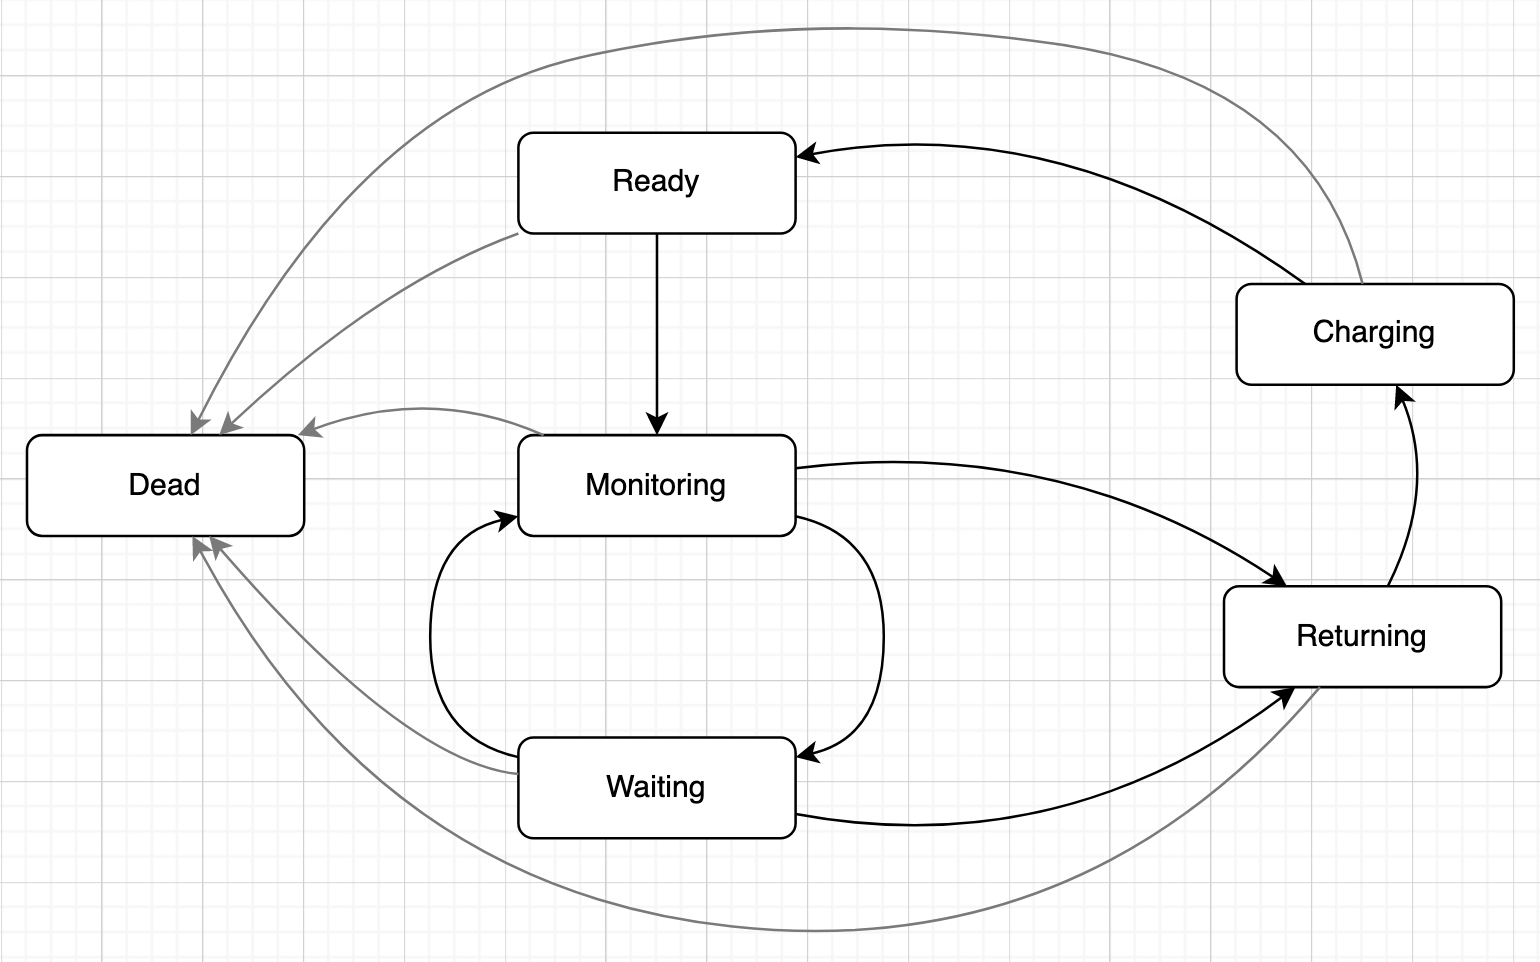
\includegraphics[height = 8 cm]{image/StateDiagram.png}
    \caption{State diagram}
\end{figure}
\subsection{Scelte progettuali}
\paragraph*{Divisione delle celle}
Dato che un punto si considera visitato se si trova nel raggio di 10 metri da un drone, possiamo discretezzare l'area rappresentandola come una matrice di celle quadrate di dimensione $10\sqrt{2} \times 10\sqrt{2}$
\begin{figure}[h]
    \centering
    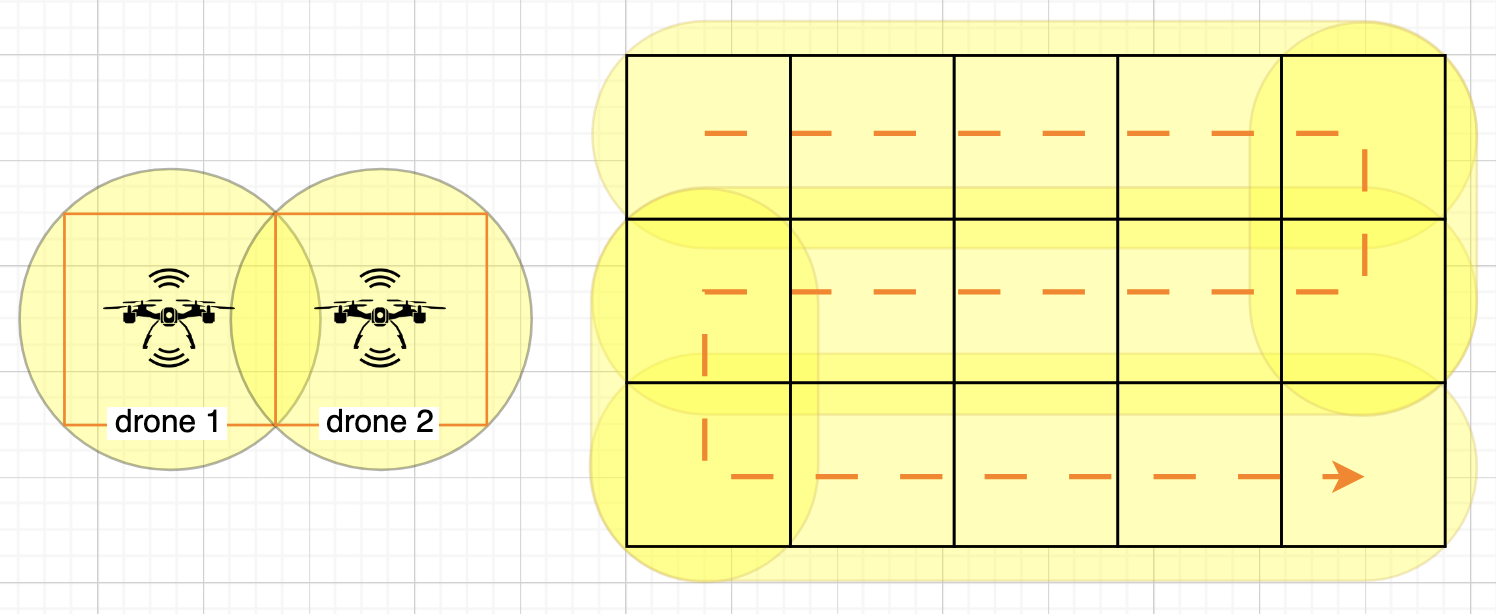
\includegraphics[height = 5 cm]{image/areedroni.png}
    \caption{L'area divisa in caselle della dimensione del quadrato inscritto nel cerchio di raggio 10}
\end{figure}
\paragraph*{Divisione dei blocchi}
Abbiamo scelto di raggruppare le caselle in blocchi circa della stessa area (la discretizzazione non garantisce la perfetta divisibilità) per garantire equità nelle assegnazioni. 
Data la variabilità delle dimensioni dell'area e del numero di droni in fase iniziale, non è sempre garantito che il numero di droni divida il numero caselle in un valore utile per costruire una matrice di blocchi.
Cerchiamo quindi due valori $h$ e $w$ tali che : $h * w > numero\ di\ droni$ e dividiamo l'area in $h\times w$ blocchi.
Questo permette a tutti i droni \textit{READY} di volare contemporaneamente all'inizio del processo di monitoraggio e quindi ridurre il più possibile il tempo di visita medio dell'intera area.
Anche se creare più blocchi ne riduce le dimensioni, questo non influisce sulle prestazioni del sistema in quanto ogni drone quando termina il ciclo di visita del suo blocco inizia a visitarne un altro e continua finché la batteria lo permette.

\paragraph*{Tempi di ricarica}
Sebbene l'algoritmo sia stato ideato per massimizzare il tempo di visita in un ciclo di carica della flotta di droni, questo non tiene conto del fatto che ogni drone può lunghi tempi di ricarica che possono superare anche di varie volte il tempo di volo di ogni drone.
Per sopperire a questo rallentamento è molto efficacie considerare la divisione in blocchi dell'area come se si avesse a disposizione solo un' $n$-esima parte dei droni.\\
Indichiamo con $n$ il numero di droni necessari per coprire il tempo di ricarica medio di un drone più uno (il tempo, medio, di volo del drone stesso). 
In questo modo si distribuisce il numero di droni in volo durante il monitoraggio a beneficio sia del tempo di visita medio che massimo.\\
Le differenze tra i vari approcci sono mostrate nella sezione risultati sperimentali.

\paragraph*{Assegnamento dei blocchi}
Per minimizzare il tempo di visita massimo e medio abbiamo sperimentato due criteri di scelta:
\begin{enumerate}
    \item \textbf{FirstAverageTime}: Assegnare ad un drone \textit{free} il blocco con tempo medio trascorso dall'ultima visita più alto (la media viene eseguita su tutte le caselle nel blocco).
    
    \item \textbf{FirstMaxTime}: Assegnare ad un drone \textit{free} il blocco che contiene la casella visitata meno di recente.
\end{enumerate}
Attualmente il programma utilizza il secondo approccio (\verb|FirstMaxTime|). Computazionalmente i due approcci sono equivalenti e dai test anche a livello di efficacia non si nota una differenza significativa 
tranne che su aree grandi con pochi droni, dove è preferibile dare più importanza al valore massimo per essere sicuri di visitare almeno una volta tutti i punti.
\section{Protocollo di comunicazione}
La Torre di Controllo ed i Droni comunicano in maniera asincrona. Le comunicazioni avvengono tramite Redis.
\subsection{Scambio di messaggi}

Ogni attore ha un suo identificativo univoco. La torre ha sempre ID = 0 mentre i droni hanno id casuali assegnati dalla torre. 
Ogni attore ha riservato un canale rappresentato su redis da una \textbf{coda} con chiave = "c:\textbf{id}"

Il proprietario usa il suo canale solo in lettura mentre gli altri attori lo utilizzano in scrittura.
Dunque ogni elemento nella coda rappresenta l'id di un messaggio con il seguente formato $(m:ID:mID)$ dove
\begin{itemize}
    \item $ID$ rappresenta l'id del mittente
    \item $mID$ rappresenta l'identificatore univoco dell'elemento nel canale.
\end{itemize}
Il contenuto di un messaggio $m$ è salvato in una \textit{HashMap} usando come chiave l'$mID$ del messaggio.
\subsection{La classe Channel}
Per gestire agevolmente la ricezione e l'invio dei messaggio è stata implementata la classe Channel, la quale gestisce un canale di un attore. Per inviare e ricevere messaggi, la classe channel presenta due metodi:
\begin{itemize}
    \item I messaggi vengono aggiunti alla coda utilizzando \verb|LPUSH c:id message_id| e salvati \\nell'HashMap con \verb|”HSET message_id {params}|
    \item In fase di lettura invece, viene utilizzato il metodo \verb|RPOP c:id| per estrarre il \verb|message_id|, e poi \verb|HGETALL message_id| per recuperarne il contenuto.
\end{itemize}
Che costituiscono le due funzioni principali per inviare e ricevere messaggi:

\textbf{void sendMessageTo(int channelId, Message \&message)}\\
Questo metodo permette di creare il messaggio su redis (quindi di creare una HashMap con $id = m:cID:mID$ e con le sue coppie $(kX,vX)$)
e di inserire l'ID del messaggio all'interno della coda.
\begin{lstlisting}[style=customcpp]
    // Creazione del messaggio su redis
    hset m:{this.id}:{message.id} {message.parseMessage()}
    
    // Aggiunta del messaggio al canale
    lpush c:{channelId} m:{this.id}:{message.id} 
\end{lstlisting}

\textbf{Message* awaitMessage(long timeout = 0)}\\
Questo metodo serve per aspettare l'arrivo di un messaggio all'interno di un canale, per poi leggerlo e ritornarlo.
Il parametro \textbf{timeout}, se diverso da -1, imposta un tempo massimo per l'attesa di un messaggio.
\begin{lstlisting}[style=customcpp]
    // Letture dell'id da redis -> restituisce un id sula variabile message_id
    BRPOP c:{this.id} timeout

    // Lettura contenuto del messaggio
    HGETALL message_id
\end{lstlisting}
\subsubsection{Thread Safety}

La Classe channel è thread safe, poiché gestisce le due funzioni \textbf{sendMessageTo} e \textbf{awaitMessage} tramite due mutex:
\begin{itemize}
    \item Un mutex in scrittura, che viene utilizzato per fare il lock durante la creazione e scrittura di un messaggio su un canale
    \item Un mutex in lettura, che viene lockato in attesa di una risposta da redis quando si tenta di leggere un messaggio dal canale.
\end{itemize}

Si è deciso di dividere le operazioni tra due mutex per questione di responsività, così che mentre un attore è in attesa di un messaggio,
possa continuare a fare altre operazioni in scrittura per aggiornare il suo stato agli occhi degli altri attori (nel nostro caso, 
torna utile per ridurre i tempi di attesa di risposta tra la torre ed i droni)
\newpage
\subsection{La classe Message}
La classe Message è la classe che rappresenta un messaggio di un canale.
\subsubsection{Costruttori e Metodi}
I costruttori della classe Message sono due:
\begin{itemize}
    
    \item \textbf{Message(std::string id)}\\
        Usato nella creazione di un messaggio già presente.
        Prende come parametro una stringa del formato \textbf{id:mid}, nel quale \textbf{id} è l'id del canale che ha inviato il messaggio, e \textbf{mid} è l'id del messaggio.

    \item \textbf{Message(int id)}\\
        Usato nella creazione di un messaggio da creare ed inviare.
        Prende come parametro un intero che rappresenta l'id del messaggio.

\end{itemize}
In aggiunta, questa classe presenta due metodi virtuali che deve implementare ogni tipo di messaggio:
\begin{itemize}
    \item \textbf{void parseResponse(RedisResponse* response)}\\
        Questo metodo serve a ricevere una Risposta da un Comando Redis, e tramutarla in messaggio. 
        La funzione prende una risposta redis che \underline{deve} essere di tipo \verb|VECTOR|, e ne legge i parametri a coppie. 
        
        Per esempio, se si leggesse un messaggio\textit{ LocationMessage}, la sua funzione di parsing legge all'interno della riposta 
        la chiave $x$, e setta la propria $x$ a quella nella risposta.
    \item\textbf{std :: string parseMessage()}\\
        Questo metodo serve a trasformare i dati contenuti nel messaggio in una stringa della forma:
        \begin{verbatim}
            type type_value p1 v1 p2 v2 p3 v3
        \end{verbatim}
        Nella quale type\_value è un intero che rappresenta il tipo del messaggio, mentre pX kX sono le coppie (parametro, valore) contenute nel messaggio

\end{itemize}



\textbf{Esempio:} LocationMessage, che serve scambiare una posizione tra drone e torre e viceversa, presenterà il corpo della funzione parseMessage() di questo tipo:
\begin{lstlisting}[style=customcpp]
    std::string LocationMessage::parseMessage() {
        std::string data = "type " + std::to_string(this->getType());
        data = data + " x " + std::to_string(this->x);
        data = data + " y " + std::to_string(this->y);
        data = data + " movement_type " + std::to_string(this->movementType);
        return data;
}
\end{lstlisting}
\subsubsection{Lista Messaggi}

% Definisce una nuova colonna di tipo "L" che è equivalente alla "l" ma più versatile per l'ambiente tabularx
\newcolumntype{L}{>{\raggedright\arraybackslash}X}

% Ridurre la dimensione del carattere della tabella
\small

\begin{adjustbox}{max width=\textwidth}
    \begin{tabularx}{\textwidth}{|L|c|L|L|}
    \hline
    \rule{0pt}{3ex} % Aggiungi spazio verticale
    \textbf{Classe} & \textbf{Tipo} & \textbf{Parametri} & \textbf{Info} \\
    \hline
    \rule{0pt}{3ex} % Aggiungi spazio verticale
    AssociateMessage & 0 & drone\_id: long long, x: int, y: int & Messaggio di associazione drone$\leftrightarrow$torre \\
    \hline
    \rule{0pt}{3ex} % Aggiungi spazio verticale
    PingMessage & 1 & nessuno & Semplice messaggio di Ping \\
    \hline
    \rule{0pt}{3ex} % Aggiungi spazio verticale
    DroneInfoMessage & 2 & \{params\} & Scambio parametri drone$\rightarrow$torre \\
    \hline
    \rule{0pt}{3ex} % Aggiungi spazio verticale
    LocationMessage & 3 & x: int, y: int & Nuova posizione per drone dalla torre \\
    \hline
    \rule{0pt}{3ex} % Aggiungi spazio verticale
    RetireMessage & 4 & nessuno & Drone con batteria scarica. Rientro necessario \\
    \hline
    \rule{0pt}{3ex} % Aggiungi spazio verticale
    DisconnectMessage & 5 & nessuno & Disconnette l'associazione drone$\leftrightarrow$torre \\
    \hline
    \end{tabularx}
\end{adjustbox}\vspace{5 mm}

\textbf{AssociateMessage}\\
Messaggio inviato dal drone alla torre per richiedere l'associazione al pool di droni.
La torre risponde ritornando l'id che associerà al drone per riconoscimento all'interno della formazione.
Il messaggio presenta il campo \textbf{drone\_id}, che rappresenta l'id temporaneo de drone in richiesta, oppure l'id associato dalla torre in caso di associazione effettuata.
Inoltre, il messaggio contiene la posizione della torre per gestire con precisione il punto di partenza dei droni.\\

\textbf{PingMessage}\\
Messaggio inviato dalla torre al drone per verificarne l'esistenza. Viene generalmente utilizzato quando la torre non riceve update dal drone per più di 2 minuti.
Questo messaggio non presenta parametri.\\

\textbf{DroneInfoMessage}\\
Messaggio per aggiornare le info di un drone all'interno del db della torre. Viene generalmente mandato dalla torre al drone, per richiedere un update dello stato del drone e verificarne il funzionamento.
I parametri del messaggio sono i campi del drone:

\indent \textbf{(\underline{drone\_id}, x, y, drone\_state, charge\_time, battery\_autonomy)}\\

\textbf{LocationMessage}\\
Messaggio con duplice scopo:
\begin{itemize}
    \item Se inviato dalla torre al drone, significa che la torre sta impostando delle nuove coordinate da raggiungere al drone. Dunque, in lettura il drone aggiornerà le coordinate e deciderà cosa fare di conseguenza.
    \item Se inviato dal drone alla torre, rappresenta un update della posizione del drone, il quale ha completato il movimento assegnatogli in precedenza.
\end{itemize}
I parametri del drone indicano sempre una posizione sul piano cartesiano (l'area da monitorare)\\

\textbf{RetireMessage}\\
Messaggio inviato dal drone per notificare la necessità di rientro per low battery.
In questo caso, la torre invia al drone un LocationMessage con le coordinate precise della torre, e lo mette in stato retiring per ottimizzare il percorso di rientro.\\

\textbf{DisconnectMessage}\\
Messaggio che rimuove l'associazione tra la torre ed il drone. Permette di liberare risorse su redis e sul database.
\newpage

\subsection{Message Sequence Chart UML}
Di seguito vengono mostrati alcuni \textbf{Message Sequence Chart UML} che mostrano i principali scenari di scambio di messaggi tra la torre e un drone qualsiasi.



\begin{tabular}{m{0.5 \textwidth} p{0.5 \textwidth}}
    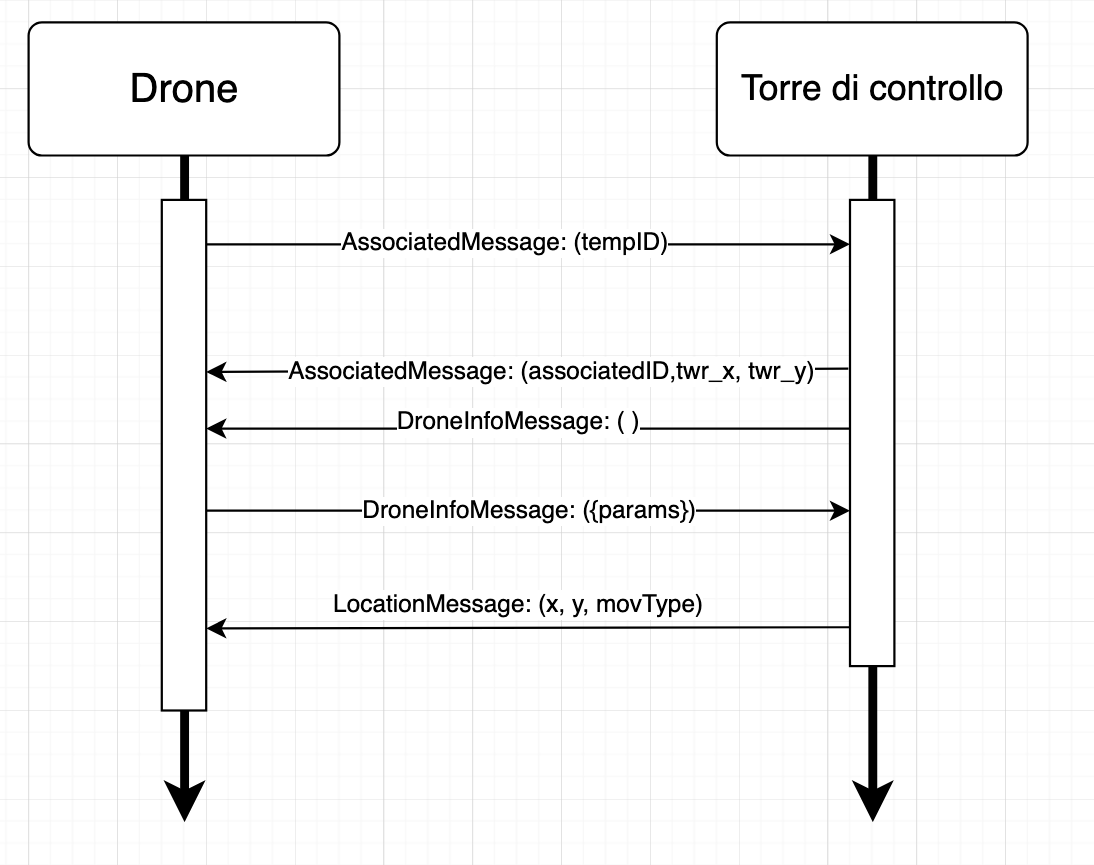
\includegraphics[width=0.45\textwidth]{image/associatedUML_MSC.png}&\textbf{Associazione di un drone:}
    \begin{enumerate}
        \item Il drone richiede di essere associato 
        \item La torre aderisce all'associazione
        \item La torre richiede le informazioni del drone
        \item Il drone risponde alla richiesta di informazioni 
        \item La torre inizia a guidare il drone 
    \end{enumerate}\\
    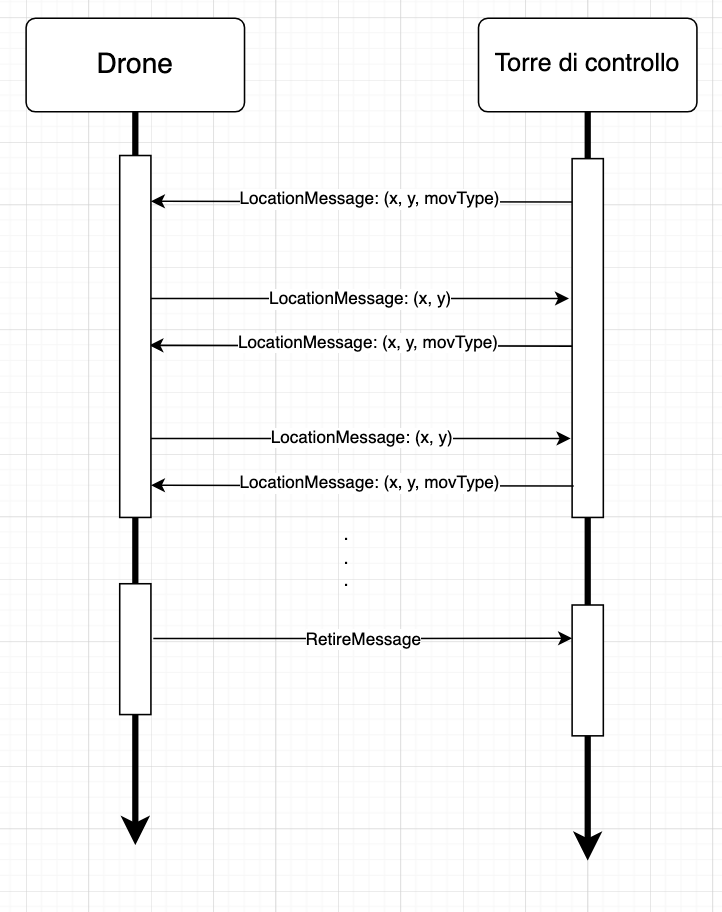
\includegraphics[width=0.45\textwidth]{image/monitoringUML_MSC.png} &\textbf{Monitoraggio di un drone:}
    \begin{enumerate}
        \item La torre invia la posizione da raggiungere
        \item Tramite il \textit{LocationMessage} il drone comunica di aver raggiunto il punto identificato
        \item La torre prontamente risponde con il nuovo punto calcolato
        \item Quando il drone non ha carica sufficiente invia un \textit{RetireMessage} e torna alla torre
    \end{enumerate}\\
    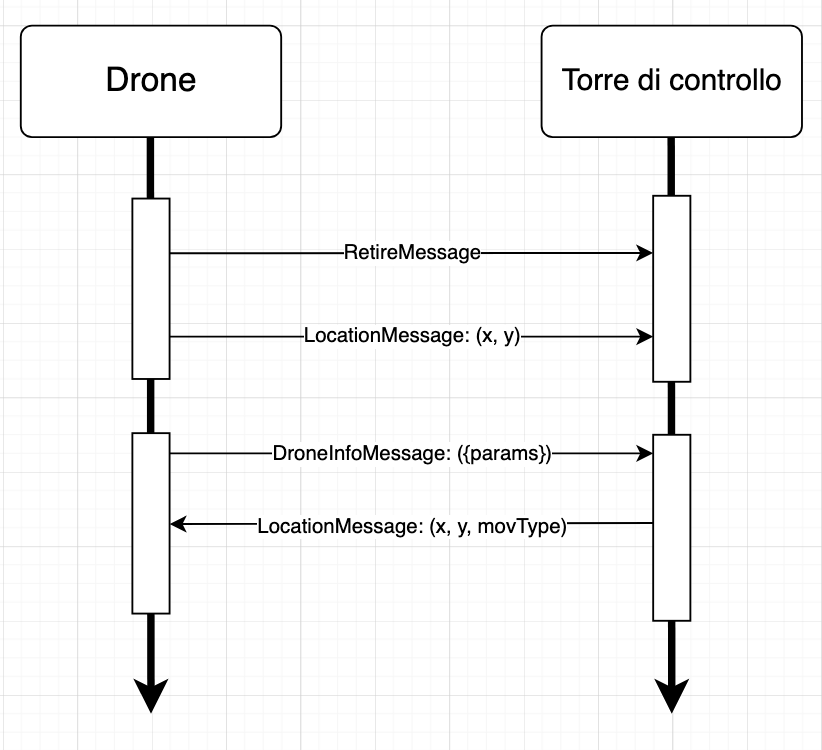
\includegraphics[width=0.45\textwidth]{image/rechargingUML_MSC.png}&\textbf{Ricarica di un drone:}
    \begin{enumerate}
        \item Il drone comunica che la sua batteria è scarica 
        \item Tramite il \textit{LocationMessage} il drone comunica di essere tornato alla torre 
        \item Il drone comunica di essersi ricaricato inviando un \textit{DroneInfoMessage}
        \item La torre ricomincia a guidarlo per monitorare l'area
    \end{enumerate}

\end{tabular}
\newpage
\section{Database}

All'interno del progetto viene sfruttato un database \textbf{PostgreSQL} per salvare dati utili in maniera persistente all'interno della torre.

\subsection{Struttura del Database}

Il Database presenta un'unica tabella: \textbf{drone}, la quale contiene le informazioni dei vari droni con il seguente schema:

\begin{longtable}{|c|c|p{0.6\textwidth}|}
\hline
\textbf{Nome} & \textbf{Tipo} & \textbf{Info} \\
\hline
id & int 64bit & Id $>$ 0 univoco del drone \\
\hline
x & integer & Coordinata x del drone all'ultimo update \\
\hline
y & integer & Coordinata y del drone all'ultimo update \\
\hline
battery\_autonomy & int 64bit & Durata della batteria all'ultimo update \\
\hline
charge\_time & int 64bit & Durata della ricarica della batteria del drone \\
\hline
dstate & int & Stato del drone all'ultimo update \\
\hline
last\_update & int 64bit & Timestamp dell'ultimo update \\
\hline
\end{longtable}

Il campo \texttt{dstate} contiene valori interi associati all'enum del codice C++:

\begin{lstlisting}[style=customcpp]
    enum DroneState {
        CHARGING,
        READY,
        WAITING,
        MONITORING,
        RETURNING,
        DEAD
    }
\end{lstlisting}

\subsection{Implementazione}

Vengono sfruttate la libreria \textbf{pqxx} per creare una connessione ed eseguire query con il database PostgreSQL.
L'eseguibile della torre prende come parametro facoltativo un file di properties, con la seguente struttura:
\begin{verbatim}
[Opzione]=Valore
\end{verbatim}
Un esempio di file base è il seguente:
\begin{verbatim}
[Ip]=http://mydomain.com/db
[User]=root
\end{verbatim}

\subsubsection{Lista DB File Properties}

\begin{longtable}{|c|c|p{0.6\textwidth}|}
\hline
\textbf{Opzione} & \textbf{Tipo} & \textbf{Info} \\
\hline
Ip & String & Ip alla connessione PostgreSQL \\
\hline
Port & Integer & Porta d'accesso del db (solo in caso di URL) \\
\hline
User & String & Username per accedere al db \\
\hline
Password & String & Password in chiaro per accedere al db \\
\hline
DbName & String & Nome del db da utilizzare \\
\hline
\end{longtable}

\textbf{NOTA:} \\
Le properties di base sono quelle di default di PostgreSQL (ip e port), con un utente chiamato \textbf{tower} senza password.

\subsubsection{Procedura di Connessione}

Una volta lette le properties, la torre crea una connessione con il db (in caso di fail, l'eseguibile si interrompe con un errore).
Una volta connessa, la torre controllerà l'esistenza della tabella \texttt{drone}, e si metterà in attesa di ricevere dei droni per iniziare il controllo dell'area.
Ogni qualvolta che un drone si connette alla torre, viene salvata la nuova entry del drone nel db.

\textbf{ID DRONE:} \\
Il protocollo di comunicazione prevede che il drone si crei un proprio id da mandare alla torre.
Di conseguenza, la torre dovrà controllare se l'id autogenerato dal drone sia valido all'interno del db (non preesistente), e in caso dovrà assegnarne uno nuovo.
\subsubsection{La tabella Blocco}
La tabella block ha senso esclusivamente nel contesto dell'algoritmo di guida dei droni pertanto seppure è presente nel diagramma ER visto in precedenza non è di interesse nel database finale.

\newpage
\section{Implementazione}
\subsection{Monitor}
seguono i monitor che assicurano che i vincoli funzionali e non-funzionali vengano rispettati
\paragraph*{locationTrigger}
Questo trigger opera sul database e assicura che ogni drone rimanga nei limiti dell'area da monitorare 
\begin{lstlisting}[language=SQL, caption={locationTrigger}]
CREATE OR REPLACE FUNCTION check_drone_area()
RETURNS TRIGGER AS $$
DECLARE
    min_x INT := 0;
    min_y INT := 0;
    max_x INT := [this->areaWidth] 
    max_y INT := [this->areaHeight]
BEGIN
    IF NEW.x < min_x OR NEW.x > max_x OR NEW.y < min_y OR NEW.y > max_y THEN
        RAISE EXCEPTION 'Drone % is out of surveillance area',
        NEW.id;
    END IF;
    RETURN NEW;
END;
$$ LANGUAGE plpgsql;
CREATE TRIGGER drone_location_check
BEFORE INSERT OR UPDATE ON drone
FOR EACH ROW
EXECUTE FUNCTION check_drone_area();
        

\end{lstlisting}
\paragraph*{batteryTrigger}
Questo trigger opera sul database e si assicura che non esistano droni che volano con la batteria scarica
    \begin{lstlisting}[language=SQL, caption={batteryTrigger}]
CREATE OR REPLACE FUNCTION check_drone_battery()
RETURNS TRIGGER AS $$
BEGIN
    IF NEW.dstate != CHARGING AND NEW.dstate != DEAD AND NEW.battery_autonomy <= 0 THEN
        'Drone % has no battery left but is still flying'
        RAISE EXCEPTION, 
        NEW.id;
    END IF;
    RETURN NEW;
END;
$$ LANGUAGE plpgsql;
CREATE TRIGGER drone_battery_check
AFTER UPDATE ON drone
FOR EACH ROW
EXECUTE FUNCTION check_drone_battery();
 
\end{lstlisting}
\newpage
\subsection{Altre parti interessanti}
Di seguito vengono riportate parti del codice implementato 
\begin{lstlisting}[style=customcpp, caption={da drone.cpp}]
    void Drone::start(float executionSpeed) {

        this->setExecutionSpeed(executionSpeed);

        // Enstablish connection to tower
        bool connectedToTower = this->connectToTower();
        if (!connectedToTower) {
            loge("Can't connect to tower!");
            return;
        }
        logi("Connected to tower");

        // Start loop
        std::thread moveThread(&Drone::behaviourLoop, this);

        std::vector<std::thread> threads;
        this->running = true;
        this->setState(READY);
        while (this->running) {
            Message *message = this->channel->awaitMessage();
            if (message == nullptr) {
                // No message received. Maybe ping tower?
                continue;
            }
            logi("Received message m:" + message->getFormattedId());
            threads.emplace_back(&Drone::handleMessage, this, message);
            // Free up completed threads
            for (auto it = threads.begin(); it != threads.end();) {
                if (it->joinable()) {
                    it ++;
                } else {
                    it = threads.erase(it);
                }
            }
        }
        // Disconnect drone
        // Wait threads to finish
        for (auto &thread : threads) {
            thread.join();
        }

    }
    \end{lstlisting}
    Il drone dopo aver completato con successo la procedura di connessione, entra in un loop in cui gestisce parallelamente sia i suoi spostamenti [riga 14.  behaviourLoop è una funzione che simula lo spostamento del drone] sia i messaggi ricevuti e da inviare alla torre di controllo.
    \newpage
    Le funzioni utilizzate per suddividere l'area in blocchi
    \begin{lstlisting}[style=customcpp, caption={da area.cpp}]

    void calculateBlocksInArea(int width, int height, int &numBlocks, int &blockWidth, int &blockHeight) {
        int w = std::sqrt(numBlocks);
        int h = w;
        while (h * w < numBlocks) {
            if ((h + 1) * w <= numBlocks) {
                h++;
            } else {
                w++;
            }
        }
        numBlocks = w * h;
        blockWidth = std::ceil(static_cast<double>(width) / w);
        blockHeight = std::ceil(static_cast<double>(height) / h);
    }

    void Area::initArea(int blockCount, int centerX, int centerY) {
        this->blocks = new std::vector<Block>();
        int blockWidth = 0;
        int blockHeight = 0;
        calculateBlocksInArea(this->width, this->height, blockCount, blockWidth, blockHeight);
        logDebug("Area", "Area Approximated to " + std::to_string(blockCount) + "(" + std::to_string(blockWidth) + "," + std::to_string(blockHeight) + ")");
        int x = 0;
        int y = 0;
        for (int i = 0; i < blockCount; i++) {
            Block b(x, y, blockWidth, blockHeight);
            x += blockWidth;
            if (b.getX() >= this->width) {
                b.setX(0);
                b.setY(b.getY() + blockHeight);
                x = blockWidth;
                y += blockHeight;
            }
            if (b.getY() >= this->height) {
                // Extra blocks
                break;
            }
            if (b.getX() + b.getWidth() >= this->width) {
                b.setWidth(this->width - b.getX());
            }
            if (b.getY() + b.getHeight() >= this->height) {
                b.setHeight(this->height - b.getY());
            }
            b.orientBlock(centerX, centerY);
            this->blocks->push_back(b);
        }
        logDebug("Area", "Fitted " + std::to_string(this->blocks->size()) + " blocks");
    }
\end{lstlisting}
\newpage
La funzione che gestisce il principale comportamento della torre
\begin{lstlisting}[style=customcpp, caption={da tower.cpp}]
    void Tower::start() {
        if (!this->channel->isUp()) {
            loge("Can't start tower without a connected channel!");
            return;
        }
        // Register signals
        signal(SIGINT, Tower::handleSignal);
        signal(SIGTERM, Tower::handleSignal);
        this->running = true;
        std::vector<std::thread> threads;
        threads.emplace_back(&Tower::droneCheckLoop, this);
        // threads.emplace_back(&Tower::areaUpdateLoop, this);
        threads.emplace_back(&Tower::drawGrid, this);
        logi("Tower online");
        while (this->running) {
            // 1' of waiting before restarting the cycle
            Message *message = this->channel->awaitMessage(10);
            if (message == nullptr) {
                // If we have no message to handle, we check last updates from drones
                // If a last update is > x second (to decide, maybe 1-5' => 60-300'') -> ping and wait a response
                // If the drone is doing nothing, we commit it to monitor a zone
            } else {
                // Handle message received on another thread, and return to listen
                logi("Received message from Drone " + std::to_string(message->getChannelId()) + ". Type: " + std::to_string(message->getType()));
                threads.emplace_back(&Tower::handleMessage, this, message);
            }
            // Free finished threads
            for (auto it = threads.begin(); it != threads.end(); ) {
                if (it->joinable()) {
                    it++;
                } else {it = threads.erase(it);}
            }
        }
        logi("Powering Off");
        // Disconnect Drones
        std::vector<Drone> drones = this->getDrones();
        for (Drone& drone : drones) {
            if (drone.droneState == DEAD) {
                continue;
            }
            DisconnectMessage *message = new DisconnectMessage(this->generateMessageId());
            this->channel->sendMessageTo(drone.id, message);
            delete message;
        }
        logi("Waiting threads to finish");
        // Await Spawned Threads
        for (auto& thread : threads) {
            thread.join();
        }
        // Flush Channel
        logi("Flushing Channel");
        bool channelFlushed = this->channel->flush();
        if (channelFlushed) {
            logi("Channel Flushed!");
        } else {
            logw("Can't flush redis channel");
        }
        logi("Printing Area");
        std::ofstream areaFile;
        areaFile.open("area.csv", std::ios_base::app);
        for(int i = 0; i < this->areaWidth; i++) {
            for(int j = 0; j < this->areaHeight; j++) {
                areaFile << this->area->operator[](i)[j] << ",";
            }
            areaFile << "\n";
        }
        areaFile.close();
        logi("Area Saved on area.scv");
    }

\end{lstlisting}
La funzione che la torre di controllo utilizza per decidere la prossima posizione da inviare ad un particolare drone
\begin{lstlisting}[style=customcpp, caption={da tower.cpp}]
    void Tower::calcolateDronePath(Drone drone) {
        // Check Active Block
        std::vector<Block> *blocks = this->area->getBlocks();
        for (Block& block : *blocks) {
            if (block.getAssignment() == drone.id) {
                // Check block cells
                if (block.getLastX() != drone.posX || block.getLastY() != drone.posY) {
                    block.setLastX(drone.posX);
                    block.setLastY(drone.posY);
                }
                int x = block.getLastX() + block.getDirX();
                int y = block.getLastY();
                if (x == this->x && y == this->y) {
                    logi("Skipping Tower Cell");
                    // Safe because the tower is in the middle
                    x += block.getDirX();
                }
                if (x >= block.getX() + block.getWidth() || x < block.getX()) {
                    y += block.getDirY();
                    x -= block.getDirX();
                    if (y > block.getY() + block.getHeight() || y < block.getY()) {
                        // Reset Block and Associate a new One
                        this->associateBlock(drone);
                        block.reset(this->x, this->y);
                        return;
                    }
                    block.setDirX(-block.getDirX());
                }
                LocationMessage *location = new LocationMessage(generateMessageId());
                location->setLocation(x, y);
                this->channel->sendMessageTo(drone.id, location);
                delete location; 
                return;
            }
        }
        // Not Returned before -> no Block associated
        this->associateBlock(drone);
    }
\end{lstlisting}

\end{document}

